\documentclass[11pt,a4paper]{article}

\usepackage[margin=1in]{geometry}
\usepackage{amsmath,amssymb,amsthm}
\usepackage{graphicx}
\usepackage{booktabs}
\usepackage{float}
\usepackage[hidelinks]{hyperref}
\usepackage{enumitem}
\usepackage{parskip}
\usepackage{multirow}

\setlength{\parindent}{0pt}

\newcommand{\R}{\mathbb{R}}
\newcommand{\E}{\mathbb{E}}

\begin{document}

% ----------------------------------------------------------------------
% Cover page
% ----------------------------------------------------------------------
\begin{titlepage}
  \centering
  \vspace*{3cm}

  {\Huge\bfseries AIST4010\par}
  \vspace{0.3cm}
  {\Huge\bfseries Foundation of Applied Deep Learning\par}
  \vspace{1.5cm}
  {\LARGE\bfseries Assignment 1\par}
  \vspace{1.5cm}
  {\Large Written Report and Code\par}
  \vspace{2cm}

  \begin{tabular}{ll}
    \Large\textbf{Name:} & \Large\rule{6cm}{0.5pt} \\[0.6cm]
    \Large\textbf{Student ID:} & \Large\rule{6cm}{0.5pt} \\[0.6cm]
    \Large\textbf{Date:} & \Large October 14, 2026 \\
  \end{tabular}

  \vfill
\end{titlepage}

% ----------------------------------------------------------------------
\section{Question 1: Derivative of the sigmoid function (10 pts)}

\textbf{Claim.}
\[
\frac{d}{dx}\,\sigma(x) \;=\; \sigma(x)\bigl(1-\sigma(x)\bigr),
\qquad\text{where}\quad \sigma(x)=\frac{1}{1+e^{-x}} .
\]

\textbf{Proof.} Write $\sigma(x) = \bigl(1+e^{-x}\bigr)^{-1}$ and apply the chain rule:
\begin{equation}
\frac{d\sigma}{dx}
= -\,\bigl(1+e^{-x}\bigr)^{-2}\cdot \frac{d}{dx}\bigl(1+e^{-x}\bigr)
= -\,\bigl(1+e^{-x}\bigr)^{-2}\cdot\bigl(-e^{-x}\bigr)
= \frac{e^{-x}}{\bigl(1+e^{-x}\bigr)^2} .
\end{equation}
Now split the right-hand side using $1+e^{-x}=\frac{1}{\sigma(x)}$:
\begin{equation}
\frac{e^{-x}}{\bigl(1+e^{-x}\bigr)^2}
= \frac{1}{1+e^{-x}}\cdot\frac{e^{-x}}{1+e^{-x}}
= \sigma(x)\left(\frac{1+e^{-x}-1}{1+e^{-x}}\right)
= \sigma(x)\left(1-\frac{1}{1+e^{-x}}\right) .
\end{equation}
Since $\frac{1}{1+e^{-x}}=\sigma(x)$, the last expression equals
$\sigma(x)\bigl(1-\sigma(x)\bigr)$, which proves the identity. $\blacksquare$

\emph{Remark:} this local smooth derivative is exactly what makes the sigmoid (and the
logistic loss) trainable with gradient-based optimization; the gradient is largest when
the model is uncertain ($\sigma\approx0.5$) and vanishes when it is saturated
($\sigma\approx 0$ or $1$).

% ----------------------------------------------------------------------
\section{Question 2: A multi-layer linear network is equivalent to a single-layer network (10 pts)}

\textbf{Claim.} A feed-forward network composed of $L$ linear (affine) layers
\[
h^{(l)}(x)=W^{(l)}h^{(l-1)}+b^{(l)},\qquad l=1,\dots,L,\quad h^{(0)}=x,
\]
has exactly the same set of representable functions as a \emph{single} affine layer
$h(x)=\tilde{W}x+\tilde{b}$.

\textbf{Proof.} By induction on $L$.

\emph{Base case} ($L=1$): trivially true.

\emph{Inductive step}: suppose a network of $L-1$ layers can be written as one affine
map, $h^{(L-1)}(x)=\hat{W}x+\hat{b}$. Then the $L$-layer network is
\[
h^{(L)}(x) = W^{(L)}\bigl(\hat{W}x+\hat{b}\bigr)+b^{(L)}
          = \underbrace{W^{(L)}\hat{W}}_{\tilde{W}}\,x
            + \underbrace{W^{(L)}\hat{b}+b^{(L)}}_{\tilde{b}}
          = \tilde{W}x+\tilde{b},
\]
where $\tilde{W}\in\R^{d_L\times d_0}$ and $\tilde{b}\in\R^{d_L}$ are again a single
matrix and bias vector, i.e.\ a single affine layer. By induction, every $L$-layer
linear network reduces to one affine layer, so the function classes coincide.
$\blacksquare$

\emph{Remark:} the composition of affine maps is affine. What an $L$-layer \emph{linear}
network gains over a single layer is nothing in expressivity -- it only adds redundant
parameters. It is the element-wise \emph{nonlinear} activations between layers that
break this equivalence and allow deep networks to represent far richer function
families than shallow ones.

% ----------------------------------------------------------------------
\section{Question 3: ROC curve and AUC (10 pts)}

The dataset contains $P=6$ positive samples (label 1) and $N=4$ negative samples
(label 0). For a threshold $t$, the classifier predicts $\hat y = 1 \iff x \geq t$.
Sweeping $t$ over the six distinct feature values gives:

\begin{table}[H]
\centering
\begin{tabular}{cccccc}
\toprule
Threshold $t$ & TP & FP & TPR = TP/6 & FPR = FP/4 & ROC point $(FPR, TPR)$ \\
\midrule
$0.9$ & 1 & 0 & $1/6$  & $0$   & $(0,\; 1/6)$ \\
$0.7$ & 3 & 1 & $3/6$  & $1/4$ & $(1/4,\; 1/2)$ \\
$0.6$ & 4 & 2 & $4/6$  & $1/2$ & $(1/2,\; 2/3)$ \\
$0.4$ & 4 & 3 & $4/6$  & $3/4$ & $(3/4,\; 2/3)$ \\
$0.3$ & 5 & 4 & $5/6$  & $1$   & $(1,\; 5/6)$ \\
$0.1$ & 6 & 4 & $1$    & $1$   & $(1,\; 1)$ \\
\bottomrule
\end{tabular}
\caption{ROC points for the threshold-based classifier on the given dataset.}
\end{table}

Connecting $(0,0)$ to these points in order and finishing at $(1,1)$ gives the
piecewise-linear ROC curve. Since the curve is a concatenation of trapezoids over the
$FPR$ axis, the AUC equals the trapezoidal sum of the TPR values:

\begin{align*}
\mathrm{AUC}
&= \tfrac{1}{2}\Big[\bigl(0+\tfrac{1}{6}\bigr)\cdot\tfrac{1}{4}
 + \bigl(\tfrac16+\tfrac12\bigr)\cdot\tfrac14
 + \bigl(\tfrac12+\tfrac23\bigr)\cdot\tfrac14
 + \bigl(\tfrac23+\tfrac23\bigr)\cdot\tfrac14
 + \bigl(\tfrac23+\tfrac56\bigr)\cdot\tfrac14
 + \bigl(\tfrac56+1\bigr)\cdot0 \Big] \\
&= \frac{1}{2}\left[\frac{1}{24}+\frac{1}{6}+\frac{7}{24}+\frac{1}{3}+\frac{3}{8}\right]
 = \frac{1}{2}\cdot\frac{7}{6}
 = \boxed{\frac{7}{12} \approx 0.5833}.
\end{align*}

(For each segment we use the trapezoid area formula
$\tfrac12(\mathrm{TPR}_{i-1}+\mathrm{TPR}_i)\cdot\Delta\mathrm{FPR}$.) This value was
double-checked numerically with \texttt{sklearn.metrics.roc\_auc\_score}, which also
returns $0.5833$. An AUC of $7/12$ is only slightly better than random guessing
($0.5$), which is consistent with a dataset whose classes overlap heavily on this
single feature.

% ----------------------------------------------------------------------
\section{Question 4: Logistic regression from scratch and in PyTorch (20 pts)}

\textbf{(a) Data generation.} \texttt{generate\_data(num\_features=100,
num\_samples=2000)} draws the inputs from a standard Gaussian and shifts the two
classes to opposite sides of a random separating hyperplane (1000 points per class,
margin 1.0). Gaussian feature noise (std $0.5$) plus $3\%$ random label flips make the
data not perfectly linearly separable. The test set is generated the same way with
\texttt{num\_samples=100} (50 per class). A fixed seed (42) is set inside the function
so results are fully reproducible. All experiments use $lr=0.001$, 100 epochs, and
initialization $W=\mathbf{0}$, $b=0$. The loss is the average binary cross-entropy.

\textbf{(b) Gradient descent (NumPy).} Full-batch GD is implemented with the
vectorized gradients $\nabla_W \mathcal L=\tfrac{1}{n}X^\top(\sigma(XW+b)-y)$ and
$\nabla_b \mathcal L=\tfrac{1}{n}\sum_i(\sigma(x_i^\top W+b)-y_i)$.
Test accuracy: $\mathbf{0.84}$. Train loss: $0.6931\to 0.6700$; test loss:
$0.6931\to 0.6680$. Final parameters: $\lVert W\rVert_2=0.0483$, $b=0.0005$. With
$lr=0.001$ the loss decreases slowly but steadily.

\textbf{(c) Stochastic gradient descent (NumPy).} SGD updates the parameters with one
sample at a time after shuffling each epoch. Test accuracy: $\mathbf{0.84}$. Train
loss: $0.6931\to 0.4219$; test loss: $0.6931\to 0.3787$. Final parameters:
$\lVert W\rVert_2=1.5297$, $b=0.0217$. As expected, SGD moves much faster than
full-batch GD (the plot shows a steeper, noisier descent).

\textbf{(d) Loss curves.} Figure~\ref{fig:q4} shows the train/test loss for GD and
SGD. Both converge without overfitting; SGD is visibly faster per epoch.

\begin{figure}[H]
\centering
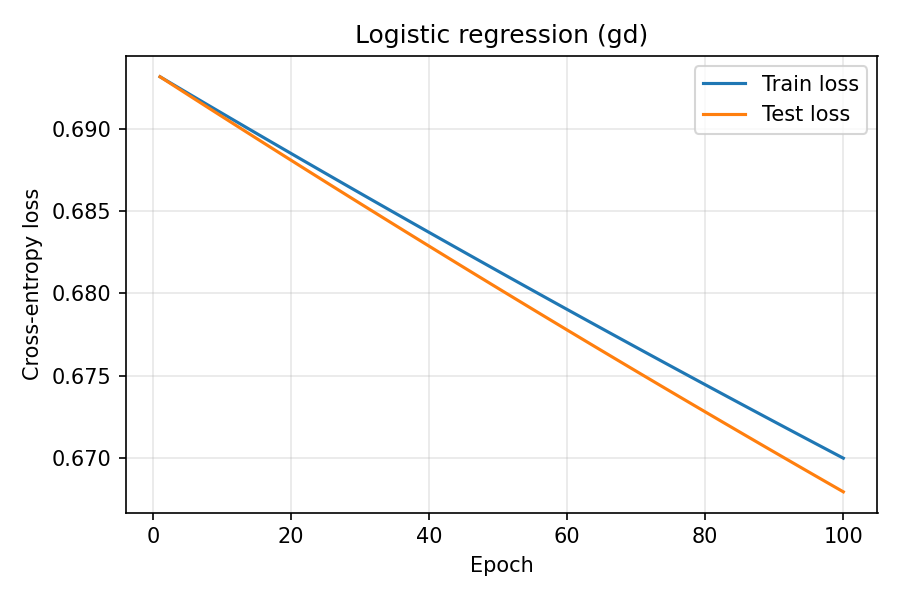
\includegraphics[width=0.47\textwidth]{../gd_loss.png}\hfill
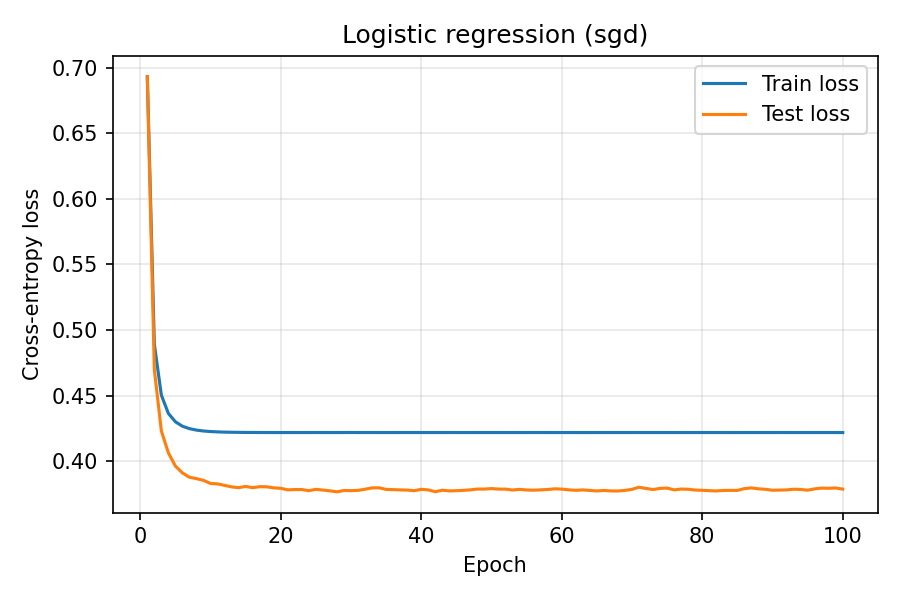
\includegraphics[width=0.47\textwidth]{../sgd_loss.png}
\caption{Q4(d): train/test cross-entropy loss of GD (left) and SGD (right),
both trained with $lr=0.001$ for 100 epochs.}
\label{fig:q4}
\end{figure}

\textbf{(e) PyTorch version.} A \texttt{torch.nn.Linear(100,1)} followed by a
\texttt{Sigmoid}, trained with \texttt{BCELoss} and \texttt{torch.optim.SGD}
($lr=0.001$) for 100 epochs. All operations are vectorized over the whole dataset
and gradients come from autograd, so there is no Python loop over samples (only the
epoch loop).
Test accuracy: $\mathbf{0.84}$. Train loss: $0.6931\to 0.6700$; test loss:
$0.6929\to 0.6677$. Final parameters: $\lVert W\rVert_2=0.0483$, $b=0.0005$.

\begin{figure}[H]
\centering
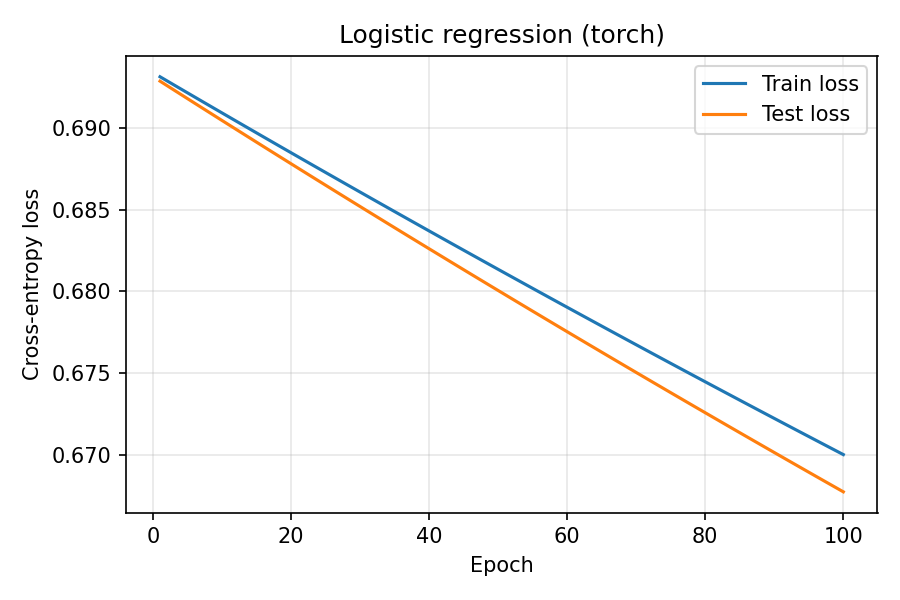
\includegraphics[width=0.47\textwidth]{../torch_loss.png}
\caption{Q4(e): train/test loss of the PyTorch logistic regression. It matches the
NumPy GD curve almost exactly (same update rule and initialization).}
\label{fig:q4torch}
\end{figure}

All three implementations reach the same $0.84$ test accuracy. The PyTorch run is
initialized at $W=\mathbf{0}$, $b=0$ (same as the NumPy runs) so that its batch
SGD update coincides with full-batch GD, which is why Figures~\ref{fig:q4} (left) and
\ref{fig:q4torch} are nearly identical.

% ----------------------------------------------------------------------
\section{Question 5: Classifiers on the Iris dataset (10 pts)}

\subsection{Experimental setup}
The 105 labeled samples from \texttt{a0/} (4 features, 3 classes) are used with
5-fold stratified cross-validation (the same folds for every model). All features are
standardized. The four models are:
\begin{itemize}[itemsep=1pt]
  \item \textbf{Logistic regression} (multinomial, \texttt{sklearn}, $L_2$ penalty);
  \item \textbf{SVM} with an RBF kernel ($C=1$, $\gamma=\mathrm{scale}$);
  \item \textbf{FCN}: fully-connected net $4\to64\to32\to3$ with ReLU, trained with
        Adam ($lr=0.05$, 300 epochs, batch 16, cross-entropy);
  \item \textbf{CNN}: 1-D convolutional net on the 4 features (2 conv layers, 16 and
        32 channels, kernel 3, then global average pooling $\to3$), same training
        recipe.
\end{itemize}

\subsection{Results}
\begin{table}[H]
\centering
\begin{tabular}{lc}
\toprule
Model & 5-fold CV accuracy (mean $\pm$ std) \\
\midrule
Logistic regression & $0.9524 \pm 0.0426$ \\
SVM (RBF)           & $\mathbf{0.9714 \pm 0.0381}$ \\
FCN ($4{-}64{-}32{-}3$) & $0.9333 \pm 0.0486$ \\
CNN (1-D)           & $0.9429 \pm 0.0356$ \\
\bottomrule
\end{tabular}
\caption{Q5: cross-validated classification accuracy on the Iris data.}
\label{tab:q5}
\end{table}

\textbf{Best model.} The RBF-kernel SVM gives the best performance
($0.9714\pm0.0381$), followed by logistic regression ($0.9524$), then the 1-D CNN
($0.9429$) and the FCN ($0.9333$). The gaps are small: with only 105 samples and 21
per fold, a single misclassified sample moves the accuracy by about $0.048$, so all
models are statistically close. The ranking SVM $>$ LR $>$ CNN $>$ FCN is consistent
with the two linear/shallow methods being best suited to this small, mostly
linearly-separable dataset.

\textbf{(6 pts for models; 4 pts for the analysis below.)}

\subsection{Why doesn't a deep neural network show its power on the Iris dataset?}
Three main reasons:

\begin{enumerate}[itemsep=2pt]
  \item \textbf{Too little data.} The Iris dataset has only 150 samples in total (105
  labeled here). Deep networks have thousands or millions of parameters and need a
  correspondingly large amount of data to estimate them; with 105 samples the FCN/CNN
  cannot be trained to their full capacity and end up memorizing or underfitting, not
  generalizing. Deep learning's advantage shows at scale, and Iris is the opposite of
  scale.
  \item \textbf{The problem is too simple.} Iris is almost linearly separable: two of
  the three classes (setosa vs.\ the others) are separated by a single hyperplane, and
  two features (petal length/width) alone nearly solve the task. A deep network exists
  to build hierarchical features for complex, high-dimensional structure (images,
  speech, text); here a linear model already captures the decision boundaries, so the
  extra layers add nothing but variance and optimization difficulty. In fact the
  linear/logistic models slightly \emph{outperform} the neural nets.
  \item \textbf{Low-dimensional input without structure.} With 4 tabular features
  there is no spatial or hierarchical structure to exploit -- no local patterns for
  convolutions, no hierarchy of abstractions. Deep learning shines on raw structured
  inputs (pixels, waveforms, tokens); on 4 numbers, a nonlinear SVM or a small
  network saturates the achievable accuracy, and the FCN's extra capacity only
  increases overfitting risk on 21-sample validation folds.
\end{enumerate}

In short: deep networks pay off when there is a lot of data and a lot of structure to
learn; Iris has neither, so a well-tuned shallow model (SVM) is the best choice.

% ----------------------------------------------------------------------
\section{Question 6: Paper summaries (40 pts)}

\subsection{ImageNet Classification with Deep Convolutional Neural Networks}

The subsection title above refers to the AlexNet paper (Krizhevsky, Sutskever and
Hinton, 2012).

\textbf{Motivation:} prior to 2012, image recognition systems were hand-engineered
feature pipelines (SIFT/HOG + SVM) that had saturated on datasets like PASCAL. The
authors wanted to test whether a large, purely learned deep CNN could finally tackle
ImageNet's 1.2M-image, 1000-class scale.
\textbf{Novelty:} the first deep CNN to win ILSVRC by a wide margin; introduced ReLU
activations (much faster to train than tanh/sigmoid), GPU-parallel training across two
GPUs, overlapping max-pooling, local response normalization, data augmentation and
dropout to fight overfitting on 60M parameters.
\textbf{Intuition:} convolutions reuse filters across the image, giving translation
invariance and far fewer parameters than MLPs, while depth learns a hierarchy of
features (edges $\to$ textures $\to$ object parts $\to$ objects); ReLU gradients don't
vanish, so a network this deep could be trained at all.
\textbf{Implementation:}
\url{https://github.com/pytorch/vision/blob/main/torchvision/models/alexnet.py}
(original CUDA code mirrored at
\url{https://github.com/dansuh17/alexnet-imagenet-sgd}).

\subsection{Deep Residual Learning for Image Recognition (ResNet)}
\textbf{Motivation:} simply stacking more layers \emph{degrades} accuracy (deeper
networks had higher training error) -- the degradation was not overfitting but an
optimization problem, so the authors sought a way to make very deep networks easy to
optimize.
\textbf{Novelty:} residual learning: each block learns $H(x)=F(x)+x$ through
identity ``skip connections''. This enables 50/101/152-layer networks (and later
1000+) that win ILSVRC 2015, COCO detection/segmentation, with a single
reformulation and no extra parameters at inference.
\textbf{Intuition:} if the target mapping is close to identity, the residual $F(x)$
is small and easy to learn; the skip connections also give gradients a direct highway
to earlier layers, preventing vanishing/exploding gradients and making the identity
mapping the default so extra depth can only help.
\textbf{Implementation:}
\url{https://github.com/pytorch/vision/blob/main/torchvision/models/resnet.py}
(original Caffe: \url{https://github.com/KaimingHe/deep-residual-networks}).

\subsection{U-Net: Convolutional Networks for Biomedical Image Segmentation}
\textbf{Motivation:} biomedical image segmentation needs pixel-level labels but only
has small annotated datasets (e.g.\ 30 microscopy images). Sliding-window networks
were slow, and plain encoder-decoder upsampling lost fine spatial detail.
\textbf{Novelty:} a symmetric encoder-decoder with skip connections that concatenate
high-resolution encoder features into the decoder, plus heavy data augmentation with
elastic deformations; wins ISBI 2012/2015 segmentation challenges with very few
images.
\textbf{Intuition:} the contracting path captures \emph{what} is in the image
(context, semantics) while the expanding path recovers \emph{where} it is; the skip
connections re-inject fine spatial information destroyed by pooling, so precise
boundaries can be reconstructed even from scarce data.
\textbf{Implementation:} \url{https://github.com/milesial/Pytorch-UNet}
(official Caffe version: \url{https://lmb.informatik.uni-freiburg.de/people/ronneber/u-net/}).

\subsection{A Simple Framework for Contrastive Learning of Visual Representations (SimCLR)}
\textbf{Motivation:} self-supervised representation learning from unlabeled images
lagged far behind supervised features, and prior contrastive methods needed
specialized architectures or memory banks. The authors wanted to identify which design
choices actually matter.
\textbf{Novelty:} a simple framework: strong stochastic data augmentation, a small
projection head $g(\cdot)$, the normalized temperature-scaled cross-entropy
(NT-Xent) loss, larger batch sizes (up to 8192) and longer training. It matches or
beats supervised ResNet-50 features on ImageNet with only 1\% labeled data.
\textbf{Intuition:} pulling augmentations of the same image together while pushing
apart different images forces the network to keep only what is invariant to nuisance
transformations -- i.e.\ semantic content; the projection head keeps this invariant
information while the representation below it is free to stay rich.
\textbf{Implementation:} \url{https://github.com/google-research/simclr}.

\subsection{Masked Autoencoders Are Scalable Vision Learners (MAE)}
\textbf{Motivation:} BERT-style masked prediction dominated NLP, but in vision the
analogous task was hard: images are spatially redundant, so reconstruction is too
easy. The authors asked whether masking and reconstruction could scale to large
Vision Transformers.
\textbf{Novelty:} an asymmetric encoder-decoder ViT: 75\% of image patches are masked
\emph{and removed}, the encoder sees only the visible patches, and a lightweight
decoder reconstructs all pixels (normalized per-patch). This trains 3--4$\times$
faster and scales to huge models, e.g.\ ViT-H/14 fine-tuned to $87.8\%$ ImageNet
accuracy.
\textbf{Intuition:} masking most patches removes spatial redundancy so the task
requires real semantic understanding; processing only visible patches cuts compute,
and the heavy lifting happens in the encoder while the cheap decoder is discarded
after pre-training, giving representations that transfer well to detection and
segmentation.
\textbf{Implementation:} \url{https://github.com/facebookresearch/mae}.

\end{document}
